\section{TIC en la educación}
\setcounter{sectiontotal}{3}

\begin{frame}[c]
    \frametitle{\pagetitle}
    \framesubtitle{Corrientes pedagógicas}

    \pause{}
\begin{columns}

\column{.5\textwidth} \hspace{0.5cm}
\begin{itemize}[<+->]
	\item Instruccionismo
	\item Conductismo
	\item Constructivismo
	\item Construccionismo
\end{itemize}

\column{.4\textwidth} \hspace{0.5cm}
\begin{overprint}
    \onslide<2|handout:1> 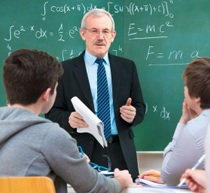
\includegraphics[width=\textwidth, height=5cm]{imagenes/tradicional} 
    \onslide<3|handout:0> 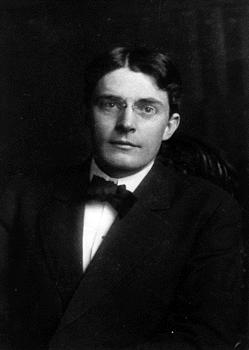
\includegraphics[width=\textwidth, height=5.5cm]{imagenes/conductismo} 
    
    \centering
    Jhon Watson
    
    \onslide<4|handout:0> 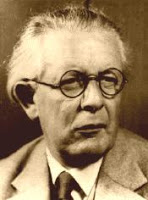
\includegraphics[width=\textwidth, height=5.5cm]{imagenes/constructivismo} 

	\centering
	Jean Piaget    
    
    \onslide<5|handout:0> 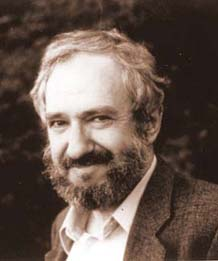
\includegraphics[width=\textwidth, height=5.5cm]{imagenes/construccionismo} 

	\centering
	Seymour Papert    
    
\end{overprint}


\end{columns}


\end{frame}

\begin{frame}
    \frametitle{\pagetitle}
    \framesubtitle{Ventajas}
    \begin{itemize}[<+->]
        \item Nuevos modelos pedagógicos\sfcite{guenaga2013serious}.
        \item Eliminación de distancias\sfcite{punie:ict}.
        \item Colaboración distribuida\sfcite{unesco:ict}.
        \item Motivación para aprender\sfcite{martin2008modelo}.
        \item Adquisición de habilidades básicas\sfcite{martin2008modelo}.
    \end{itemize}
\end{frame}

\begin{frame}
    \frametitle{\pagetitle}
    \framesubtitle{Desafíos}
	 \begin{itemize}[<+->]
        \item Falta de motivación de los profesionales\sfcite{punie:ict}.
        \item Altas expectativas\sfcite{punie:ict}.
        \item Brecha social\sfcite{punie:ict}.
        \item Aspectos financieros\sfcite{unesco:ict}.
    \end{itemize}
\end{frame}
